% Nejprve uvedeme tridu dokumentu s volbami
\documentclass[czech,bachelor]{diploma}
% Dalsi doplnujici baliky maker
\usepackage[autostyle=true,czech=quotes]{csquotes} % korektni sazba uvozovek, podpora pro balik biblatex
\usepackage[backend=biber, style=iso-numeric, alldates=iso]{biblatex} % bibliografie
\usepackage{dcolumn} % sloupce tabulky s ciselnymi hodnotami
\usepackage{subfig} % makra pro "podobrazky" a "podtabulky"
\usepackage[cpp]{diplomalst}
\usepackage{dirtree}

% Zadame pozadovane vstupy pro generovani titulnich stran.
\ThesisAuthor{Jan-Kryštof Zahradník}

\ThesisSupervisor{Ing. Lukáš Klein}

\CzechThesisTitle{Navržení a implementace rezervačního systému pro posilovny s ohledem na maximální kapacitu, typ tréninku a využití nástrojů}

\EnglishThesisTitle{Design and Implementation of a Booking System for Gyms with Regard to Maximum Capacity, Type of Training and Use of Tools}

\SubmissionYear{2024-2025}

\ThesisAssignmentFileName{ThesisSpecification_ZAH0089.pdf}

% Pokud nechceme nikomu dekovat makro zapoznamkujeme.
\Acknowledgement{Rád bych zde poděkoval vedoucímu této práce Ing. Lukáši Kleinovi za pomoc a cenné rady při tvorbě této bakalářské práce}

\CzechAbstract{Tato bakalářská práce se zaměřuje na návrh a implementaci rezervačního systému pro posilovny s důrazem na správu kapacity, typů tréninků a dostupných zdrojů. Výsledkem je webová aplikace, která uživatelům umožňuje rezervovat jednotlivé posilovací stroje v konkrétním čase, navrhovat vhodné stroje odpovídající jejich tréninkovým plánům a optimalizovat čas tréninku na základě zvoleného počátečního času.}

\CzechKeywords{rezervační systém; posilovna; webová aplikace; bakalářská práce}

\EnglishAbstract{This bachelor's thesis focuses on the design and implementation of a reservation system for gyms, emphasizing efficient management of capacity, training types, and available resources. The result is a web application that allows users to book individual exercise machines at specific times, suggest suitable machines that align with their training plans, and optimize training schedules based on the selected start time.}

\EnglishKeywords{reservation system; gym; web application; bachelors thesis}

\AddAcronym{API}{Application Programming Interface}
\AddAcronym{REST API}{Representational State Transfer API}
\AddAcronym{JS}{JavaScript - Programovací jazyk}
\AddAcronym{TS}{TypeScript - Programovací jazyk}
\AddAcronym{ORM}{Objektově relační mapování}
\AddAcronym{PK}{Primární klíč}
\AddAcronym{FK}{Cizí klíč}
\AddAcronym{HTTP}{HyperText Transfer Protocol}
\AddAcronym{CI}{Continuous integration - kontinuální integrace}
\AddAcronym{CD}{Continuous deployment - kontinuální vydávání}
\AddAcronym{a pod.}{A podobně}
\AddAcronym{atd}{a tak dále}

\addbibresource{citations.bib}

% Novy druh tabulkoveho sloupce, ve kterem jsou cisla zarovnana podle desetinne carky
\newcolumntype{d}[1]{D{,}{,}{#1}}


% Zacatek dokumentu
\begin{document}

% Nechame vysazet titulni strany.
\MakeTitlePages

% Jsou v praci obrazky? Pokud ano vysazime jejich seznam a odstrankujeme.
% Pokud ne smazeme nasledujici dve makra.
\listoffigures
\clearpage

% Jsou v praci tabulky? Pokud ano vysazime jejich seznam a odstrankujeme.
% Pokud ne smazeme nasledujici dve makra.
\listoftables
\clearpage

% A nasleduje text zaverecne prace.
\chapter{Úvod}
\label{sec:Introduction}
V současné době převažují ve fitness komunitě rezervační systémy odlišné od návrhu představeného v této bakalářské práci. Stávající řešení se primárně zaměřují na rezervaci osobních tréninků s certifikovanými trenéry nebo na alokaci prostoru pro skupinové aktivity, jako jsou spinningové lekce, boxerské tréninky či jiné specializované kolektivní programy. Tyto rezervační systémy však nedostatečně řeší problém přetížení fitness center, který se výrazně projevuje zejména v období zvýšené poptávky (např. na začátku roku). Následkem toho jsou návštěvníci nuceni průběžně upravovat své tréninkové plány podle aktuální dostupnosti přístrojů a kapacity zařízení, což snižuje jak efektivitu tréninku, tak celkovou spokojenost klientů.

Hlavní limitace současných systémů tkví v neschopnosti dynamicky reagovat na vytíženost jednotlivých přístrojů. Místo toho, aby monitorovaly stav zařízení v reálném čase (např. obsazenost běžeckých pásů, činek nebo strojů). To vede k nerovnoměrnému vytížení vybavení, častým časovým překryvům a nevyužitým kapacitám v méně frekventovaných časech.

Tento problém je mimořádně komplexní, protože je nutné zohlednit nejen maximální kapacitu posilovny, ale také vyhnout se kolizím v používání jednotlivých přístrojů. Na trhu i v open-source komunitě momentálně neexistuje žádné podobné řešení, které by tento problém řešilo efektivním a škálovatelným způsobem.

Tato bakalářská práce se zaměřuje na návrh a implementaci rezervačního systému pro posilovnu, který inteligentně doporučuje vhodné časy a přístroje pro jednotlivé uživatele. Výsledkem je REST API s webovou aplikací, která umožňuje uživatelům intuitivně spravovat své rezervace a získávat optimální doporučení pro jejich tréninkové plány.
\endinput

\chapter{Popis použitých technologií}

Tato kapitola se zaměřuje na technologie využité při vývoji systému popsaného v této bakalářské práci. Jednotlivé technologie jsou zde představeny v kontextu jejich funkce v rámci využití napříč vrstvami v systému. Cílem této části je poskytnout čtenáři přehled o nástrojích a prostředích, které byly zvoleny, a zároveň objasnit důvody, proč byly konkrétní technologie preferovány před jinými.

Ústřední roli v celém ekosystému hraje JavaScript, který se stal jádrem celého vývojového procesu. Tato volba vycházela z mnoha později uvedených důvodů, ale i přesto, že odpovídá široce rozšířené praxi, byla klíčová pro volbu ostatních technologií.

Tato bakalářská práce prošla několika vývojovými iteracemi. V klíčových změnách týkajících se výběru technologií mezi těmito různými verzemi systému bude podrobně pojednáno v části nazvané změněné technologie. Konečný soubor technologií zahrnuje následující technologie: 
\begin{itemize}
    \item \textbf{Backend}
        \begin{itemize}
            \item PostgreSQL
            \item JavaScript/TypeScript
            \item Node.js
            \item Express.js
        \end{itemize}
    \item \textbf{Frontend}
        \begin{itemize}
            \item Vue.js
            \item Tailwind CSS
            \item ShadCN
            \item Clerk
            \item Zod
        \end{itemize}
    \item \textbf{Testy \& CI/CD}
        \begin{itemize}
            \item Docker
            \item Git / Github
            \item CI/CD - Github Actions
            \item Python \& pytest
        \end{itemize}    
\end{itemize}

V následujících podkapitolách jsou proto jednotlivé technologie detailně popsány včetně jejich výhod, nevýhod a konkrétního využití v rámci systému.

\section{JavaScript}
JavaScript je základním stavebním kamenem praktické implementace této bakalářské práce. Byla v něm i napsána úplně první verze celého backendu. V projektu byl JS použit z několika důvodů:

\begin{description}
  \item[Rozšířená komunita] \hfill \\ JS má obrovskou komunitu vývojářů, která nabízí bohatou podporu a nespočet open-source knihoven a frameworků, což usnadňuje a zrychluje vývoj \cite{dev52MDevelopers}.
  \item[Nativní podpora ve webových prohlížečích] \hfill \\ I v dnešní době, kdy máme mnohem více možností, je JS stále "Jazykem webu"\cite{ranjan2020javascript} a běží nativně ve všech moderních prohlížečích\cite{browserstackJavaScriptCode}, což z něj činí téměř nezbytnou součást vývoje webových aplikací. Pro jednoduchost a jednotu mezi vrstvami dávalo smysl používat jeden jazyk.
\end{description}

Použití JavaScriptu umožnilo rychlý start a flexibilní rozvoj projektu. Samozřejmě, že jeho volba s sebou přinesla i některé problémy a úskalí, se kterými se bylo potřeba v průběhu vývoje vypořádat. Tímto se budeme detailněji zabývat v kapitole \ref{retrospective}.

V pozdější části implementace došlo k rozhodnutí přejít na \texttt{TypeScript}, což byl důležitý krok směrem k lepší struktuře a stabilitě kódu.

\subsection{TypeScript}
Je to open-source programovací jazyk vyvíjený společností Microsoft \cite{typescriptlangDocumentationTypeScript}, který je postavený na JavaScriptu a rozšiřuje ho o typovou kontrolu\cite{goldberg2022learning}. TS poskytuje výhodu především ve větších projektech, kde je potřeba zajistit stabilitu a minimalizovat chyby spojené s dynamickým typováním JavaScriptu.

Statická typová kontrola v TS umožňuje odhalit chyby již během psaní kódu a nabízí větší jistotu při refactoringu \cite{enwiki:1258410189, sethi1996programming}. Přestože TS stále generuje běžný JavaScript, přináší strukturovanější a bezpečnější vývojový proces, což významně zlepšilo kvalitu kódu.

\section{PostgreSQL}
PostgreSQL je open-source objektově-relační databázový systém, který byl v této práci zvolen jako databázové řešení \cite{postgresqlPostgreSQL}. Tento databázový systém je známý svou stabilitou, rozšiřitelností a podporou pokročilých funkcí, jako jsou uložené procedury, transakce nebo plná podpora ACID (Atomicita, Konzistence, Izolace, Trvalost). PostgreSQL nabízí škálovatelnost a spolehlivost, které jsou klíčové pro náročné webové aplikace.

Prvotní verze byla vytvořena s použitím MySQL, protože jsem s touto technologií v minulosti již pracoval. Migrace na PostgreSQL proběhla kvůli možnosti využití bezplatného hostingu. Aplikace byla zpočátku vyvíjena na různých zařízeních a usiloval jsem o zachování datové konzistence bez nutnosti migračního systému. Nakonec tento požadavek vymizel a s ním i potřeba hostovat databázi mimo lokální prostředí. Nyní databáze běží v Docker kontejneru.

\section{Node.js}
Pro spuštění a chod programu potřebují programovací jazyky specifické běhové prostředí (Ang. Runtime environment)\cite{enwiki:1245152116, alfred2007compilers}. Při vývoji JavaScriptu byl vytvořen ``JavaScript engine'' pro webový prohlížeč Netscape Navigator. V podstatě se jednalo o velmi jednoduchý interpretor. Později se tento engine vyvinul v SpiderMonkey, který je dodnes používán v prohlížeči Mozilla Firefox \cite{newJavaScriptEngineModuleOwner}. Alternativa pro Chromium se nazývá V8\cite{v8JavaScriptEngine}.

Node.js poskytuje běhové prostředí pro JavaScript mimo prohlížeč. Vznikl v roce 2009 a umožnil použití JavaScriptu pro serverové aplikace. Je postaven na enginu V8 a díky tomu je velmi výkonný a efektivní.\cite{nodejsNodejsAbout}

Node.js je dnes největším běhovým prostředím pro JavaScript na světě. Kromě možnosti tvorby serverových aplikací poskytuje ekosystém balíčků spravovaný přes \texttt{npm}(Node Package Manager), což je největší repozitář softwarových balíčků na světě.\cite{npmjsAboutDocs}

Mezi alternativy patří například \texttt{Bun} a \texttt{Deno}, avšak \texttt{Node.js} stále představuje průmyslový standard, což je i důvod, proč byl zvolen pro tuto práci \cite{chhetri2016comparative}.

\section{Express.js}
Express.js je minimalistický webový framework pro Node.js, který byl použit pro tvorbu aplikačního programového rozhraní (API). Express usnadňuje práci s HTTP metodami a nabízí jednoduchou, ale flexibilní strukturu pro vývoj REST API\cite{expressjsExpressNodejs}.

Express umožňuje jednoduchou, ale transparentní práci s HTTP metodami, z něhož tvoří oblíbenou volbu pro vývoj webových aplikací všech velikostí. V této práci byl využit pro tvorbu REST API, které funguje jako komunikační most mezi frontendem a databází.

\section{Vue.js}
Vue.js je progresivní open-source framework pro tvorbu uživatelských rozhraní\cite{vuejsVuejs}. Byl zvolen pro frontend tohoto projektu díky své jednoduchosti a flexibilitě. Vue.js umožňuje rychlý vývoj komponent, které jsou zabaleny do velmi přehledné struktury.

Hlavní silnou stránkou Vue.js je jeho reaktivní systém správy stavu. Tento mechanismus automaticky sleduje závislosti mezi daty a rozhraním, což eliminuje potřebu explicitního řízení aktualizací \cite{vuejsVuejsDocs}.

Frameworky jako React používají imperativní správu stavu pomocí hooků (např. useState) \cite{bugl2019learn}, \texttt{Vue.js} umožňuje přímou mutaci reaktivních proměnných deklarovaných pomocí \texttt{ref()} nebo~\texttt{reactive()} \cite{vuejsVuejsDocs}. Tento rozdíl redukuje boilerplate kód a snižuje riziko chyb spojených s nesprávnou synchronizací stavu. Následující ukázka demonstruje implementaci čítače v Reactu s použitím hooku \texttt{useState}:
\begin{lstlisting}
function Example() {
  const [count, setCount] = useState(0);
  return (
    <div>
      <p>You clicked {count} times</p>
      <button onClick={() => setCount(count + 1)}>
        Click me
      </button>
    </div>

  );
\end{lstlisting}
Zde je nutné explicitně deklarovat jak stavovou proměnnou (count), tak odpovídající setter (setCount). Každá změna stavu vyžaduje volání setter funkce, což vede k přerenderování komponenty. Ačkoli tento model poskytuje granularitu kontroly, vyžaduje od vývojáře důsledné oddělení stavové logiky a prezentace. Naproti tomu stejná funkcionalita ve Vue.js využívá reaktivní referenci:
\begin{lstlisting}
<script setup>
import { ref } from "vue";
const counter = ref(0);
</script>

<template>
  <div>
    <p>You clicked {{ counter }} times</p>
    <button @click="counter++">Click me</button>
  </div>
</template>
\end{lstlisting}
Proměnná \texttt{counter} je obalena proxy objektem, který automaticky detekuje změny prostřednictvím getterů a setterů generovaných funkcí \texttt{ref()}. Mutace hodnoty přímým přiřazením (counter++) spouští reaktivní aktualizaci DOM bez nutnosti manuálního volání setterů.

\section{Tailwind CSS}
Tailwind je framework pro CSS, který výrazně zrychluje stylování uživatelského rozhraní \cite{tailwindcssTailwindRapidly}. Namísto tradičních předpřipravených komponent nabízí Tailwind množství utility tříd, které lze kombinovat a vytvářet tak design přímo v HTML komponentách.

Použití Tailwindu v tomto projektu umožnilo vytvořit flexibilní a rychle upravitelný design bez nutnosti psát samotné CSS.

\section{Shadcn}
Shadcn je sada komponent výhradně pro React a Tailwind, která zjednodušuje integraci uživatelského rozhraní do aplikací. Umožňuje rychlé nasazení a styling komponent pomocí Tailwind CSS, čímž snižuje čas potřebný na vývoj frontendu. Jedná se o předem nastylované Radix komponenty \cite{shadcnIntroduction}.

Na rozdíl od ostatních sad komponent, jako například Bootstrap, shadcn přidá kód komponent přímo do projektu, tudíž jsou plně upravitelné. Vue komunita vytvořila svou neoficiální verzi Shadcn s názvem Shadcn-vue, která byla v této práci využita \url{https://www.shadcn-vue.com/}.

Použití této knihovny komponent ulehčilo vývoj webového uživatelského rozhraní s dodáním celistvého vzhledu.

\section{Clerk}
Clerk je autentizační a správcovská služba uživatelů, která zjednodušuje implementaci přihlašování, registrací a správy uživatelů v aplikacích. Nabízí snadnou integraci s frontendovými technologiemi, jako je Vue.js\cite{clerkClerkAuthentication}. 

V tomto projektu je Clerk použit pro autentizaci, což zajišťuje bezpečný přístup k aplikaci.

\section{Zod}
Zod je knihovna pro validaci dat. Umožňuje definovat schémata, která popisují tvar dat, a následně je validovat \cite{zodTypeScriptfirstSchema}.

V tomto projektu je Zod využíván k validaci dat přicházejících ze shadcn formulářů. Tímto zajišťuje konzistenci a správnost dat na serverové straně.

\section{Docker}
Docker je nástroj, který slouží k vývoji, distribuci a spouštění aplikací. Umožňuje oddělit aplikace od infrastruktury, což usnadňuje a zrychluje nasazování softwaru. Díky Dockeru se dá infrastruktura spravovat podobně jako aplikace. Pomocí metod, které Docker nabízí pro testování, nasazování a~distribuci kódu, se dá zkrátit čas mezi napsáním kódu a jeho spuštěním v ostrém provozu\cite{a2024_what}.

V rámci tohoto projektu Docker poskytuje efektivní a rychlé řešení, které umožňuje vývoj a~distribuci aplikace napříč různými platformami.

\section{Git / Github}
Git je distribuovaný systém pro správu verzí, který umožňuje efektivní sledování změn a správu různých verzí souborů. Je široce využíván díky své flexibilitě a podpoře týmové spolupráce, čímž se stal standardem mezi verzovacími systémy \cite{spinellis2012git}.

V této bakalářské práci byl Git nasazen od počátku jako klíčový nástroj pro verzování. Pro sdílení a správu repozitáře byl zvolen GitHub, populární platforma rozšiřující Git o funkce pro ukládání, správu a spolupráci v cloudu. Díky svému intuitivnímu prostředí se GitHub stal oblíbeným řešením pro projekty všech velikostí \cite{githubAboutGitHub}.

\section{CI/CD - Github actions}
GitHub Actions je platforma pro kontinuální integraci a doručování (CI/CD), která umožňuje automatizovat procesy, jako jsou sestavení, testování a nasazování aplikací. S GitHub Actions lze vytvářet pracovní postupy, které automaticky sestaví a otestují každý pull request v repozitáři, nebo nasadí sloučené pull requesty přímo do produkce\cite{githubinc_2024_understanding}.

Při vývoji rezervačního systému byly GitHub Actions především použity pro vytvoření Docker kontejneru a pro spuštění testů.

\section{Python a pytest}
Python je vysoce úrovňový interpretovaný skriptovací jazyk, který se vyznačuje unikátním způsobem strukturování kódu. Namísto tradičního používání složených závorek pro seskupování bloků kódu využívá Python bílých znaků (whitespace), což přispívá k jeho čitelnosti a jednoduchosti \cite{kuhlman2009python, van1990functional}.

V rámci tohoto projektu je Python využit pro vývoj API testů, přičemž byl využit framework pytest. Pytest je vcelku jednoduchý a s kombinací s možností rychlého vývoje v Pythonu toto technologické rozhodnutí umožnilo opravdu rychlý vývoj jednoduchých testů.


\chapter{Teoretická analýza} \label{theoreticalAnalysis}
Tato kapitola se věnuje teoretickému návrhu systému, jehož cílem je optimalizace rezervací tréninkových časů a využití posilovacích přístrojů ve fitness centru. Klíčovým záměrem je definice algoritmických principů pro tři základní funkce systému, které tvoří jeho logické jádro:

\begin{enumerate}
    \item \textbf{Doporučení přístrojů} - Systém by měl umět doporučit vhodné doplňující přístroje a to na základě již zvolených zařízení.
    \item \textbf{Generování času pro trénink} - Na základě zadaného počátečního času a dostupnosti jednotlivých přístrojů musí systém navrhnout časový harmonogram jejich využití, přičemž zohlední kapacitní omezení a možný souběh rezervací.
    \item \textbf{Doporučení nejbližších časů} - Při manuální konfiguraci časových oken je třeba detekovat případné kolize s ostatními rezervacemi a na základě této analýzy navrhnout nejbližší dostupné časové okno stejné délky.
\end{enumerate}

Před samotným rozborem jednotlivých algoritmických přístupů je nezbytné vymezit základní terminologii, která bude v této kapitole dále používána:
\begin{enumerate}
    \item \textbf{Rezervace} - Konkrétní záznam o rezervaci tréninku. Je vázaná na datum, tréninkový plán a~konkrétního uživatele. Může být navíc asociována s trenérem.
    \item \textbf{Rezervace} - Tréninkový plán, který definuje posloupnost přístrojů, jejich časové alokace, typ tréninku a případně další parametry.
    \item \textbf{Přístroj} - Konkrétní zařízení používané při cvičení (např. leg press, běžecký pás, atd.).
\end{enumerate}

Pro lepší orientaci a detailnější uvedení do kontextu je potřeba definovat postup, jakým bude uživatel interagovat s těmito algoritmy. Vytvoření rezervace bude probíhat skrze konfigurační formulář, který bude zaobalovat tento následující postup, viz Activity diagram procesu vytvoření rezervace. \ref{fig:ReservationActionDiagram}
\begin{itemize}
  \item Zákazník vyplní základní informace ohledně rezervace.
    \begin{itemize}
      \item Mezi základní informace se započítává například datum rezervace, název plánu a počet osob, atd.
    \end{itemize}
  \item Zákazník může vybrat trenéra
  \item Systém vyhledá všechny přístroje dostupné v posilovně
  \item Zákazník vybírá přístroje, dokud nevybere všechny, které chce.
    \begin{itemize}
        \item Pokud zákazník vybere více než určený počet přístrojů (např. 3), tak systém začne doporučovat přístroje, jež jsou spojeny s typem tréninku, který v dosavadním výběru přístrojů převažuje. V tomto kroku se odehrává \textbf{Doporučení přístrojů}
    \end{itemize}
  \item Zákazník si zvolí, zda chce konfigurovat časová okna manuálně.
      \begin{itemize}
        \item Pokud ne, tak systém zablokuje možnost vybírat pořadí přístrojů. Zákazník si vybere počáteční čas a systém vygeneruje jednotlivá časová okna, která následně doplní do jednotlivých položek. Zde se odehrává \textbf{Generování času pro trénink}. Dále může časová okna ještě poupravit. 
        \item Pokud ano, tak uživatel zvolí pořadí přístrojů. Následně zákazník volí časová okna pro jednotlivé přístroje. 
    \end{itemize}
    
  \item Během manuálního vkládání/upravování časových oken systém kontroluje, zda v zadaném časovém okně je kolize s jinou rezervací. Pokud je, tak systém vyhledá nejbližší volné okno stejné délky před a po zvoleném úseku. Zde se bude odehrávat \textbf{Doporučení nejbližšího dostupného času}.
  \item Nakonec zákazník zvolí dodatečné informace, jako například kategorie tréninku atd.
\end{itemize}

\begin{figure}
    \centering
    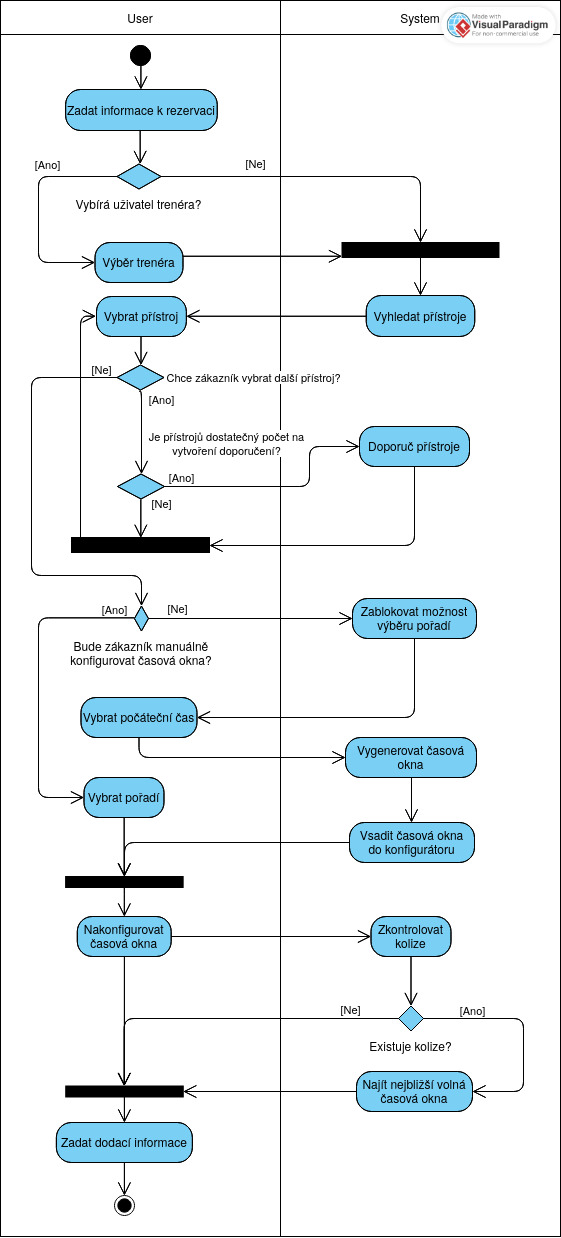
\includegraphics[width=.5\textwidth]{Figures/Bakalarka, rezervace.jpg}
    \caption{Action diagram procesu vytvoření rezervace}
    \label{fig:ReservationActionDiagram}
\end{figure}

\section{Doporučení přístrojů}
Doporučení přístrojů na základě jejich typu je vcelku jednoduché. Nejprve je nutné určit, pro jaký typ tréninku se budou přístroje doporučovat. To zajistíme tak, že budeme mít informaci o možných typech tréninku někde uloženou, konkrétně v databázi. 

Systém tedy projde každý vybraný přístroj, zjistí, jaké typy tréninku jsou na přístroji možné, a~ten, který se vyskytuje nejčastěji, bude považovat za cílový trénink, který zákazník chce navolit. Na základě nalezeného typu tréninku tedy systém najde všechny přístroje, které tento typ sdílí, a~podle jejich popularity vybere někol2ik nejpopulárnějších. 

Problémy s kolizemi v tuto chvíli není potřeba u doporučování přístrojů řešit. Systém nebude mít ve chvíli, kdy bude zákazník přístroje vybírat, kontext o tom, kdy se trénink bude odehrávat.

\section{Doporučení nejbližšího dostupného času}
Doporučení nejbližšího času je již komplexnější. Problematika spočívá v detekci kolizí a v hledání časového okna, které je stejné délky, jež nekoliduje s žádnou další rezervací, a to jak před zvoleným časovým oknem, tak i po něm.

Uživatel bude schopen si také povolit, nebo zakázat kolize na jednotlivých přístrojích. Například je pro systém žádoucí mít neustále povolené kolize na činkách, jelikož jich je mnoho. Kolize se budou řešit úplně stejně jako případy bez kolizí, jen s tím rozdílem, že u kolizí bude systém navíc kontrolovat kapacitu. Pokud bude souběžný počet lidí na jednom přístroji v mezích jeho kapacity, tak systém považuje toto časové okno jako volné; pokud ne, tak ho považuje jako zabrané. Uživatel bude na existující kolizi upozorněn, ale nebude se jednat o stav blokující ho ve vytvoření rezervace.

Systém nejprve načte existující rezervace daného přístroje pro zvolené datum a extrahuje z nich počáteční a koncové časy všech rezervovaných časových oken. Tato okna jsou následně seřazena vzestupně podle počátečního času, čímž vzniká chronologický přehled obsazených intervalů. Před zahájením analýzy systém předpokládá, že uživatelem zadané časové okno splňuje základní validaci – počáteční čas je chronologicky před koncovým časem.

Následně systém porovná vstupní časové okno s uspořádaným seznamem rezervací a identifikuje první interval, který s ním koliduje (překrývá se). Jakmile je kolize detekována, algoritmus vyhledá nejbližší volný interval mezi již existujícími rezervacemi před konfliktním oknem, jehož délka odpovídá nebo přesahuje požadovanou dobu trvání. Stejný postup aplikuje i na intervaly za konfliktním oknem, čímž získá dvě potenciální alternativy: první volné okno před a druhé po původně zvoleném čase.

Pro lepší představu se lze odkázat na diagram \ref{fig:ReservationTimeSuggestionDiagram}. Každá bílá buňka reprezentuje zabraná časová okna, červená ty, se kterými zadaný interval koliduje, šedá ty, která jsou moc krátká, a zelená ty, jež jsou vhodná pro doporučení. 

\begin{figure}
    \centering
    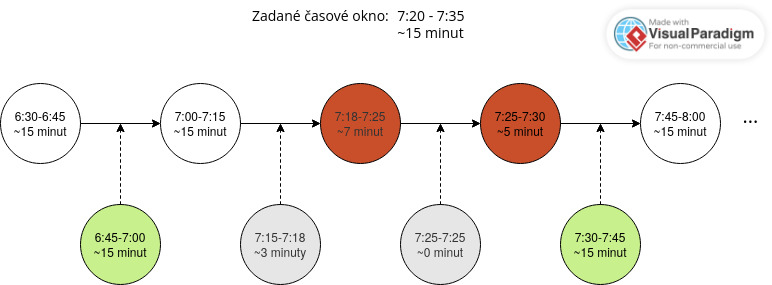
\includegraphics[width=1\textwidth]{Figures/time_suggestion_diagram.jpg}
    \caption{Diagram nalezení nejbližších volných časových oken}
    \label{fig:ReservationTimeSuggestionDiagram}
\end{figure}

\section{Generování času pro trénink}
Generování tréninků je z předem zmíněných možností asi nejkomplexnější. Problematika spočívá v tom, že nejenže musíme najít vhodné časy, ale opět řešit kolize a to vše, aby byl trénink bez prázdných časových oken, ve kterých zákazník nemá zarezervovaný nějaký přístroj.

Nejprve je potřeba systém v určitých směrech omezit. Například bude velmi složité a neefektivní nechat uživatele zvolit pořadí přístrojů, v tu chvíli by nejen nabylo řešení na komplexitě, ale~také~by to omezilo systém v ohledu flexibility, což má být jeden z jeho klíčových aspektů. Zároveň nám zablokování možnosti měnit pořadí otevírá dveře k více flexibilnímu řešení, u kterého může pořadí přístrojů měnit sám systém tak, aby výsledný trénink byl časově efektivní a zabránil tvorbě mezer.

Dále systém umožní uživateli si vypnout, či zapnout kolize s ostatními lidmi, co kolize zapnuté mají. Tyto kolize jsou řešeny podobně jako u doporučení nejbližšího dostupného času. Nakonec dostaneme od uživatele počáteční čas. 

Generování časových oken bude řešeno pomocí grafů s neváženými směrovými hranami, kde každý vrchol grafu reprezentuje časové okno. Výsledkem je několik průchodů tohoto grafu, chápáno jako několik možností pro uživatele. Graf je skládán podle zadaných parametrů, průchod grafem je neměnný. 

\subsection{Tvorba Grafu - vrcholy}
Data v grafu vycházejí z využití vybraných přístrojů pro daný den počínaje uživatelem zadaným časem. Je nutné v datech zachovat i ty záznamy, které mají kolize vypnuté, jelikož budou důležité pro tvorbu vrcholů.

Jakmile systém získá záznamy o vytížení přístrojů, je potřeba tato data upravit do požadovaného formátu. Tento formát musí obsahovat počáteční a koncový čas časového okna, který reprezentuje. Dále je potřeba  zachovat informace o přístroji a rezervaci. Následně tato data systém upraví ještě jednou a to tím způsobem, že si doplní záznamy o mezery, tj. časová okna, přes která nikdo nemá vytvořenou rezervaci pro daný přístroj. Tyto záznamy tedy nebudou obsahovat rezervaci. 

Data budeme tedy následovně upravovat na základě vstupních hodnot poskytnutých uživatelem. Konkrétně, zda uživatel povolí kolize s ostatními uživateli, kteří tuto možnost také povolili.

Pokud uživatel kolize nepovolí, tak se nabízí zcela jednoduché řešení. Z předem připravených dat jednoduše odstraníme ty možnosti, které obsahují rezervaci, tj. někdo přes toto časové okno již rezervaci má. Tyto data budou tedy výslednými vrcholy pro tento scénář.

V případě, že uživatel kolize povolí, bude problém o něco složitější. Nejprve z právě těch záznamů, které obsahují rezervaci a zároveň mají kolize povolené, systém musí danou rezervaci odstranit, tímto se z těchto záznamů stanou předem zmíněné mezery. Rezervace, pro které nejsou kolize povoleny, zůstávají v datech zachovány. Dále systém projde všechny tyto mezery a spojí je dohromady.
Tímto se nám zmenší počet vrcholů, přes které systém poté bude procházet. Až po spojení mezer systém odstraní záznamy, jež obsahují zbývající rezervace.

Výsledkem obou případů jsou volná časová okna, která jsou pro danou konfiguraci dostupná, právě tyto hodnoty budou hodnotou vrcholů, jež v grafu budou.

\subsection{Tvorba Grafu - hrany}
Pro vytvoření hran v grafu se systém řídí dvěma základními podmínkami.

Následující podmínky využívají 2 vrcholy, vrchol A je právě ten vrchol, ze kterého má směřovat hrana, a vrchol B je kandidát na vrchol, do kterého hrana směřuje.
\begin{enumerate}
    \item Koncový čas vrcholu B musí být větší, než počáteční čas vrcholu A.
    \item Přístroj asociovaný s vrcholem A nesmí být stejný jako přístroj asociovaný s vrcholem B
\end{enumerate}

Pokud tyto dvě podmínky systém aplikuje na všechna nalezená časová okna, tak výsledkem budou potřebné hrany, skrz které se bude algoritmus pro průchod pohybovat.


\subsection{Průchod grafem}
Na průchod grafem se nabízí spousta možností, jako jsou například: DFS, BFS, Dijkstra a podobně \cite{tarjan1972depth, bundy1984breadth, javaid2013understanding}. Tyto algoritmy se dají využít na spoustu use-case, ale pro tuto implementaci bude ideální tvorba vlastního řešení.

Průchod grafem bude řešen pomocí rekurze. Princip rozhodování dalšího vrcholu bude jednoduchý. Následující vrchol bude první prvek ze vzestupně seřazené množiny podle koncového času, který nebyl dosud navštíven, a zároveň neobsahuje přístroj, jenž byl navštíven a časově se do vrcholu vejde.

Průchod grafem je vizualizován v obrázku \ref{fig:graph_walk}. S ohledem na přehlednost bylo v tomto příkladu vynecháno zobrazení všech možných hran mezi všemi vrcholy. Zobrazují se pouze hrany pro současný vrchol. Zelenou barvou jsou vyhrazeny hrany, jež jsou vybrány pro další průchod. Vpravo od grafu jsou informace k přístrojům a současný čas.

\begin{figure}
	\centering
	\subfloat[Hrany pro první vrchol přístroje s identifikátorem 1\label{fig:graph_walk_1}]
	{
		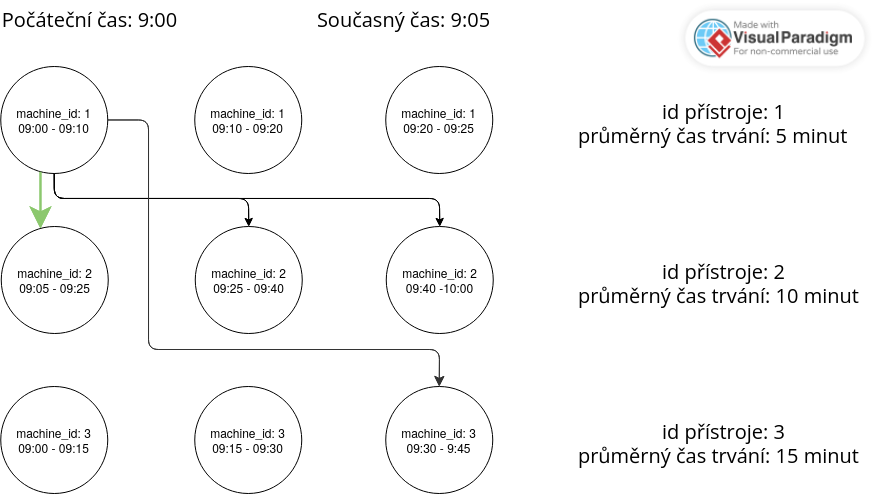
\includegraphics[width=0.9\textwidth]{Figures/Flow1.png}
	}
	\vspace{2em} % make more space
	\subfloat[Hrany pro vybraný vrchol v grafu\label{fig:graph_walk_2}]
	{
		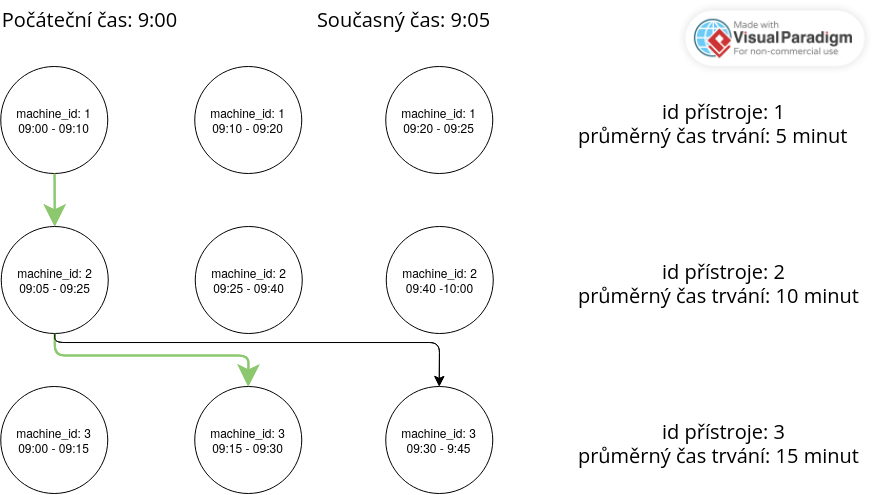
\includegraphics[width=0.9\textwidth]{Figures/Flow2.png}
	}
	\caption{Ukázkový průchod grafem pro 3 vybrané přístroje s počátečním časem 9:00}
	\label{fig:graph_walk}
\end{figure}

\chapter{Infrastruktura}

\section{Úvod}
S výjimkou databázového systému je aplikace rozdělena do dvou oddělených vrstev: frontend a backend. Rozhodnutí nevyužít fullstack framework, jako je například Nuxt, je poměrně jednoduché. Tyto dvě vrstvy mohou fungovat zcela odděleně, což umožňuje využití různých verzí technologií a zajišťuje větší flexibilitu při správě a nasazování jednotlivých částí systému.

Toto rozdělení přináší také zásadní výhody z hlediska budoucí rozšiřitelnosti. Aplikace se dá snadno přizpůsobit pro různé platformy – například ji lze rozšířit o mobilní nebo desktopovou aplikaci, aniž by to narušilo stávající strukturu. Díky této modularitě je architektura systému robustnější a lépe připravená na budoucí požadavky. Navzdory rozdělení je projekt uložený v jednom git repozitáři.

\section{Databáze}

% \subsection{Specifikace zadání}

\subsection{Vize}
Navrhovaný systém pro posilovnu bude zajišťovat správu rezervací, uživatelů a vybavení posilovny. Hlavním účelem systému je rezervační konfigurátor, jehož primární funkcí je alokace dostupných přístrojů. Systém integruje algoritmus pro dynamické doporučení optimálních časových intervalů na základě vytíženosti zařízení a přizpůsobený výběr přístrojů na bázi typu tréninku.

\subsection{Role}
Rolí systém podporuje několik. Uživatele rozdělujeme do tří skupin.

\begin{description}
    \item[Zákazník] je role s nejnižšími právy. Zákazník bude representovat osobu, která si v systému bude chtít vytvořit rezervaci
    \item[Trenér] je role která má rozšítěný přístup k systému, je to obyčejný uživatel, který může být přiřazen k rezervaci. Asociaci s rezervací může ale sám zrušit. V zadání tuto roli nemáme popsanou, tudíž se pro tento typ účtu nebude v rámci této bakalářské práce implementovat logika navíc. Prozatím bude fungovat jako obyčejný uživatel, kterého lze přidat k rezervaci jako trenéra.
    \item[Zaměstnanec] je role, která má přístup k administraci, je to role s nejvyššími právy a je schopna přidávat, manipulovat a mazat veškerá data. Bude také mít přístup ke všem statistikám a výpisům.
\end{description}
Tyto skupiny nám zajistí integritu přístupu dat a jejich manipulaci. Pro tento systém není potřeba více rolí, jelikož Zaměstnanců, kteří jsou pověřeni manipulací dat a přístupu do administrace je malé množství, tudíž téměř neomezený přístup k datům má nízké chybové dopady.

\subsection{Popis}
Systém bude primárně zaměřen na chod posilovny, což zahrnuje správu rezervací přístrojů na konkrétní časy a potenciálně i sledování výdělků. Pro zajištění těchto specifikací je potřeba se ujistit, že systém tyto specifikace pokrývá. Systém je postaven na třech pilířích.

\begin{description}
    \item[Uživatelské účty] Většina záznamů v systému vyžaduje uchovávání informací o uživateli. Samotná autentizace a související procesy, jako je ověřování uživatelů, budou řešeny mimo rámec databáze pomocí externích služeb. Nicméně je stále potřeba ukládat dodatečné informace o uživatelích přímo v databázi. Pro tento účel systém obsahuje jednoduchou tabulku s názvem account, která slouží k uchování základních informací o uživatelských účtech, jako jsou identifikátory nebo další nezbytné údaje.
    \item[Rezervace a plán] Jak napovídá samotný název, tabulka rezervace reprezentuje uživatelovu rezervaci, která je vždy vázána na konkrétní den. Každá rezervace je spojená s uživatelem a určitým plánem a může mít přiřazeného trenéra. Plán představuje komplexnější strukturu několika tabulek, které uchovávají podrobné informace o rezervaci, například konkrétní přístroje, časové rozvrhy a další detaily. Plán je tvořen následujícími tabulkami: plan, plan\_category a plan\_machine.
    \item[Přístroje a kategorie] Tabulka machine reprezentuje skutečné posilovací přístroje dostupné v posilovně. Každý přístroj má definované základní informace, jako jsou jeho název a popis, a je spojen s určitým plánem. Vztah mezi přístroji a plánem je typu N:M (mnoho na mnoho), což umožňuje asociaci jednoho přístroje s více plány a naopak. Tento vztah je dále rozšířen o dodatečné informace, jako je počet opakování (repetic), počet sérií (setů) a časové intervaly, zahrnující počáteční a koncový čas cvičení. Dále jsou s každým plánem a přístrojem asociovány kategorie, které jsou uchovávány v tabulce plan\_category. Tyto kategorie umožňují lépe strukturovat a organizovat přístroje a plány podle typu cvičení nebo jiných kritérií, což usnadňuje správu systému, zvyšuje jeho přehlednost a poskytne možnost doporučit Přístroje podle předem vybraných.
\end{description}


\subsection{Datová analýza}

\begin{figure}[h!]
	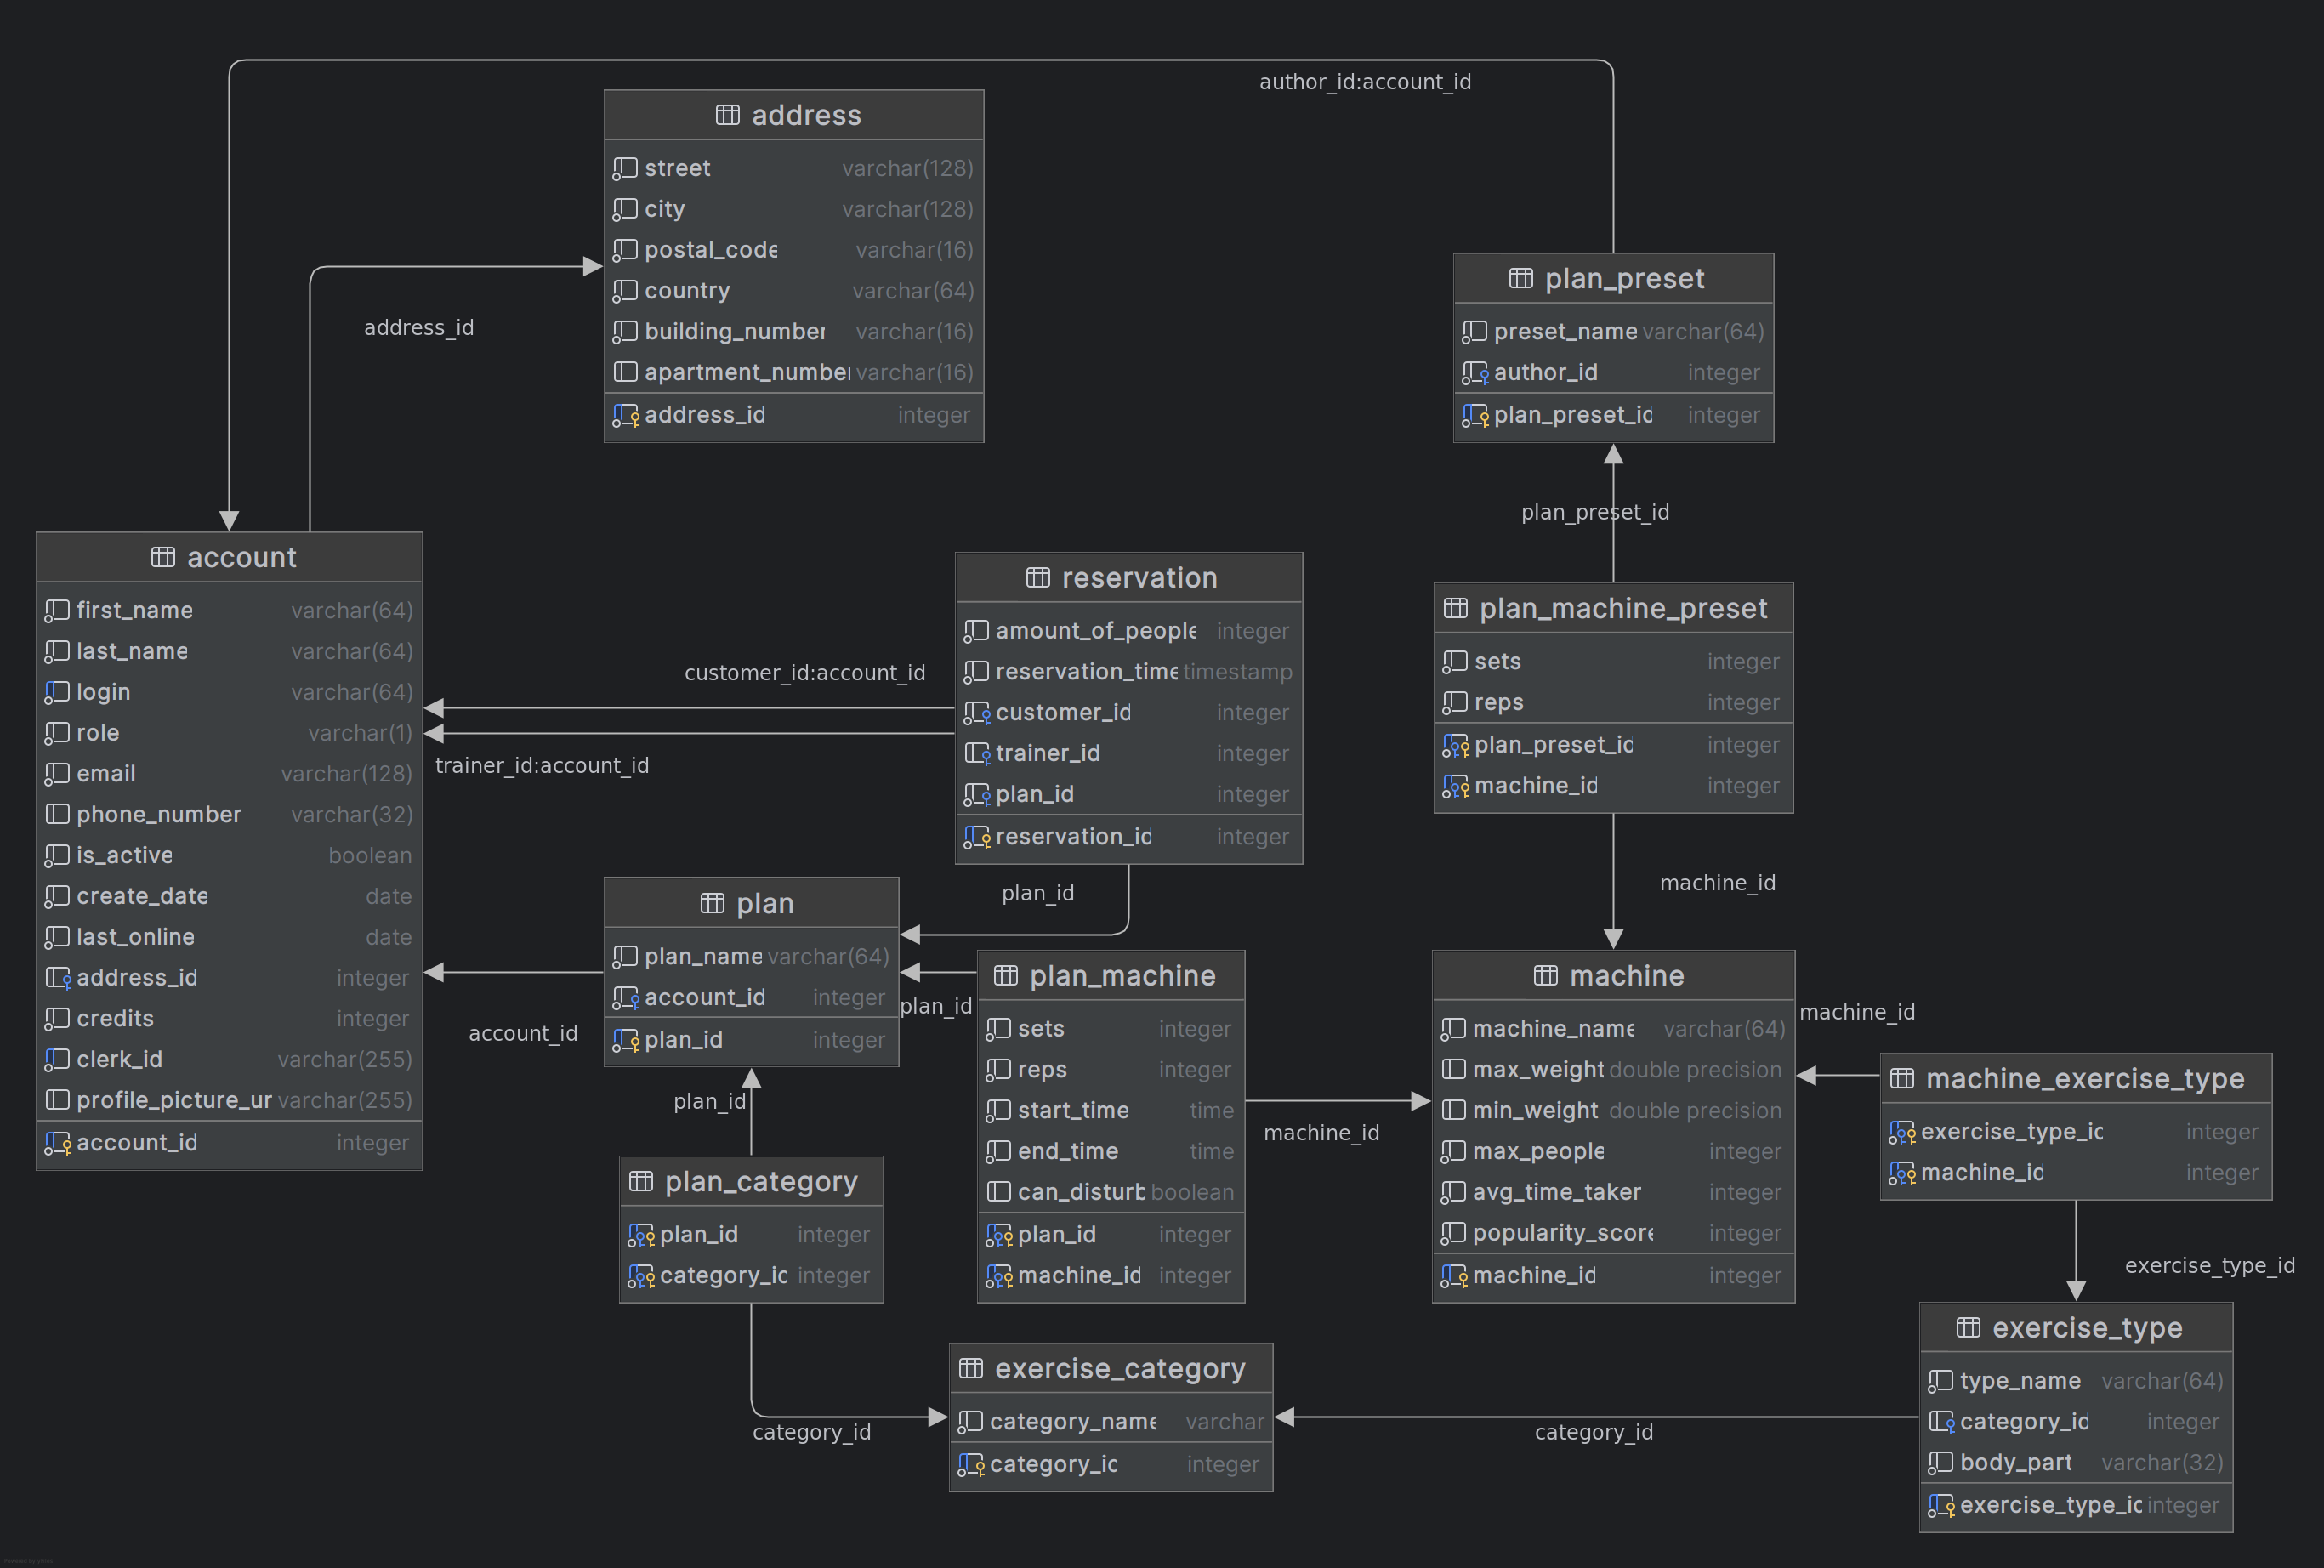
\includegraphics[width=1\textwidth]{Figures/ermodel.png}
	\caption{ Relační model}
	\label{fig:RelationalModel}
\end{figure}

\subsubsection{Popis dat}
Tato sekce se věnuje popisu nejdůležitějších tabulek, které můžeme vidět v ER-modelu. Jedná se o následující 4 tabulky: reservation (rezervace), machine (přístroj), plan (tréninkový plán), plan\_machine (slouží jako vztah mezi přístrojem a plánem, můžeme chápat jako reprezentaci časového okna). Ostatní tabulky slouží primárně k uchovávání doplňujících informací nebo ke správě relací mezi výše uvedenými tabulkami.

\begin{table}[h!]
	\caption{Popis databázové tabulky - reservation}
    \label{tab:dat-dictionary-reservation}
	\begin{tabular}{|p{3.5cm}|p{2cm}|p{1cm}|p{2.5cm}|p{.75cm}|p{3.75cm}|}
		\hline
        \textbf{Název atributu} & \textbf{Dat. Typ} & \textbf{Délka} & \textbf{Klíč} & \textbf{Null} & \textbf{Popis} \\
        \hline
        reservation\_id & INTEGER & - & Primární & Ne & Id rezervace \\
        \hline
        ammout\_of\_people & INTEGER & - & - & Ne & Počet lidí \\
        \hline
        reservation\_time & DATE & - & - & Ne & Čas příchodu \\
        \hline
        customer\_id & INTEGER & - & Cizí (account) & Ne & Id uživatele, na kterého je rezervace napsaná \\
        \hline
        trainer\_id & INTEGER & - & Cizí (account) & Ano & Id trenéra \\
        \hline
        plan\_id & INTEGER & - & Cizí (plan) & Ne & Id plánu \\
        \hline
	\end{tabular}
\end{table}

\begin{table}[h!]
	\caption{Popis databázové tabulky - machine}
    \label{tab:dat-dictionary-machine}
	\begin{tabular}{|p{3.5cm}|p{2cm}|p{1cm}|p{2.5cm}|p{.75cm}|p{3.75cm}|}
		\hline
        \textbf{Název atributu} & \textbf{Dat. Typ} & \textbf{Délka} & \textbf{Klíč} & \textbf{Null} & \textbf{Popis} \\
        \hline
            machine\_id & INTEGER   &  -    & Primární       & Ne & Id stroje \\
            \hline
            machine\_name     & VARCHAR   &  64   & -                 & Ne & Název stroje \\
            \hline
            max\_weight       & FLOAT   &  -   & -                 & Ne &  Maximální váha, kterou lze použít \\
            \hline
            min\_weight       & FLOAT   &  -    & -                 & Ne &  Minimální váha, kterou lze použít \\
            \hline
            max\_people       & INTEGER   &  -  & -                 & Ne & Maximální počet lidí na stroji \\
            \hline
            avg\_time\_taken    & INTEGER   &     & -                 & Ne & Průměrný trávený čas \\
            \hline
            popularity\_score & INTEGER      &  -    & -                 & Ne &  Počet rezervací \\
        \hline
	\end{tabular}
\end{table}

\begin{table}[h!]
	\caption{Popis databázové tabulky - plan}
    \label{tab:dat-dictionary-plan}
	\begin{tabular}{|p{3.5cm}|p{2cm}|p{1cm}|p{2.5cm}|p{.75cm}|p{3.75cm}|}
		\hline
        \textbf{Název atributu} & \textbf{Dat. Typ} & \textbf{Délka} & \textbf{Klíč} & \textbf{Null} & \textbf{Popis} \\
        \hline
            plan\_id & INTEGER   &  -    & Primární       & Ne & Id plánu \\
        \hline
            plan\_name     & VARCHAR   &  64   & -                 & Ne & Název plánu \\
        \hline
            account\_id     & INTEGER   &  -   & Cizí (account)                 & Ne & Id uživatele, který vytvořil plán \\
        \hline
	\end{tabular}
\end{table}

\begin{table}[h!]
	\caption{Popis databázové tabulky - plan\_machine}
    \label{tab:dat-dictionary-plan-machine}
	\begin{tabular}{|p{3.5cm}|p{2cm}|p{1cm}|p{2.5cm}|p{.75cm}|p{3.75cm}|}
		\hline
        \textbf{Název atributu} & \textbf{Dat. Typ} & \textbf{Délka} & \textbf{Klíč} & \textbf{Null} & \textbf{Popis} \\
        \hline
            plan\_id        & INTEGER   &  -    & Cizí (plan)       & Ne & Id plánu \\
        \hline
            machine\_id     & INTEGER   &  -    & Cizí (machine)       & Ne & Id stroje \\
        \hline
            sets                & INTEGER   &  -   & -                 & Ne & počet sérií\\
        \hline
            reps                & INTEGER   &  -    & -                 & Ne &  Počet opakování \\
        \hline
            start\_time     & TIME      &  -    & -                 & Ne & Čas začátku \\
        \hline
            end\_time       & TIME      &  -    & -                 & Ne & čas konce \\
        \hline
            can\_disturb          & BOOLEAN   &  =    & -                 & Ne & povolení kolizí \\
        \hline
	\end{tabular}
\end{table}

\subsubsection{Procedury a funkce}
Konkrétní procedury a funkce budou popsány v pozdější části této práce. Klíčovým aspektem návrhu je určení, které operace budou efektivnější realizovat na úrovni databáze a které na aplikační vrstvě. Toto rozhodnutí je zásadní, protože ovlivňuje nejen efektivitu a přehlednost řešení, ale také jeho dlouhodobou udržovatelnost.

Procedury a funkce jsou v kontextu navržené architektury využity pro extrakci komplexních datových struktur, nejsou však aplikovány pro jiné operace, jako například manipulace s daty, nebo~složitější transakce. Toto rozhodnutí vychází ze dvou východisek:

\begin{description}
    \item[Minimalizace funkcionality databázové vrstvy] 
    Databáze je využita především jako stabilní uložiště dat a optimalizovaný nástroj pro jejich vyhledávání. Transformace dat a obchodní logika je delegována na aplikační vrstvu.
    \item[Využití výhod aplikační vrstvy]
    Výhodou aplikační vrstvy oproti vrstvě datové je možnost využití obecných programovacích jazyků (např. JavaScript), které – na rozdíl od databázového jazyka PL/pgSQL – poskytují širší spektrum nástrojů pro manipulaci s daty, implementaci procedurální logiky a správu komplexních operací.  
\end{description}
Tento přístup přesouvá složitou obchodní logiku z databázové vrstvy do prostředí, které lépe odpovídá požadavkům na moderní softwarový vývoj. Zároveň toto rozhodnutí reflektuje princip separace zodpovědnosti (Separation of Concern - SoC), čímž ustanovuje jasné hranice mezi aplikační a datovou vrstvou, které následně vedou k více robustnímu a bezpečnému řešení. \cite{de2002importance}




\section{Backend}
Jedná se o HTTP rozhraní, které zajišťuje komunikaci mezi databází a uživatelským rozhraním. Rozhraní je napsáno v jazyce TypeScript, což přispívá k jazykové konzistenci napříč celým systémem a umožňuje využití moderních jazykových funkcí, včetně silné typové kontroly.

Pro práci s databází nebyly použity žádné existující knihovny pro implementaci ORM (Object-Relational Mapping). Místo toho jsem se rozhodl vytvořit vlastní implementaci ORM. Tento přístup poskytuje větší flexibilitu a kontrolu nad způsobem, jakým jsou data spravována a manipulována. Konkrétní detaily této implementace budou popsány v následujících sekcích.

\subsection{ORM}
Pro implementaci ORM jsem se rozhodl využít kombinaci reflexe a dekorátorů. Toto řešení mi umožnilo výrazně zjednodušit vývoj jednoduchých CRUD(tj. Create, Read, Update, Delete) operací pro jednotlivé koncové body. Výhodou tohoto přístupu je, že stačí definovat model, opatřit ho vhodnými dekorátory, a samotné mapování na SQL se následně provádí automaticky díky reflexi.

Důvodem rozhodnutí implementace vlastního ORM byla snaha o minimalizaci externích knihoven a jiných závislostí na straně backendu. Tento přístup poskytuje řadu výhod, například: lepší kontrolu nad kódem i jeho kvalitou, jednoznačnou zodpovědnost za případné chyby a mnohé další.

Konkrétní implementační detaily budou popsány v následující části.

\subsubsection{Dekorátory}
Dekorátory umožňují rozšířit funkcionalitu běžných tříd pomocí metadat nebo různých nadstaveb, které „dekorují“ danou třídu nebo její atributy\cite{TSDecorators}. V kontextu této práce byly tyto dekorátory implementovány přímo pro potřeby projektu, zejména pro přesné mapování objektových modelů na databázové tabulky a sloupce. Mezi naimplementovanými dekorátory vznikajícími přímo pro tuto architekturu lze rozlišit několik typů:
\begin{description}
    \item[Table] 
    Tento dekorátor slouží k přiřazení názvu tabulky dané třídě. Pomocí reflexe je název tabulky propojen s třídou, která ji reprezentuje, což usnadňuje práci při mapování modelů na SQL.
    \item[PrimaryKey]  
Dekorátor, který specifikuje primární klíč tabulky. Aplikace jej využívá pro identifikaci a práci s primárním klíčem záznamů v databázi.

\item[Column] 
Tento dekorátor přidává k atributům třídy odpovídající názvy sloupců v databázi. Zároveň přiřazuje daným atributům i specifické datové struktury v pozadí.

\item[ForeignKey] 
Dekorátor určený pro označení cizího klíče. Do dekorátoru se předává typ reprezentující odkazovanou tabulku, přičemž atribut, na který je dekorátor aplikován, musí být stejného typu. Navíc je nutné, aby odkazovaný typ dědil z obecné třídy \texttt{Model}.

\item[UnInsertable]
Označuje atributy, které mají být při vkládání dat do databáze ignorovány. Je využíváno pro zamezení vložení atributu, jejichž hodnota je nastavována skrze základní hodnoty v databázi. Například create\_date v tabulce account.

\item[DifferentlyNamedForeignKey]  
Používá se v případě, kdy atribut reprezentuje cizí klíč, ale jeho název se liší od názvu primárního klíče v odkazované tabulce. Tento dekorátor řeší situace, kdy databázová struktura neodpovídá standardnímu pojmenování. Například mějme cizí klíč \texttt{customer\_id}, který odkazuje na tabulku \texttt{account}, jenže PK má v dané tabulce název \texttt{account\_id}.

\item[UnUpdatable]  
Podobně jako \texttt{UnInsertable} tento dekorátor zajišťuje, že atributy označené tímto dekorátorem budou ignorovány při požadavku aktualizace dat.

\item[ManyToMany]
Dekorátor, který označuje atributy reprezentující vztah typu M:N (mnoho na mnoho) mezi dvěma tabulkami. Tento dekorátor umožňuje automatické zpracování spojovacích tabulek a souvisejících operací.
\end{description}


\subsection{Struktura}
Struktura projektu prošla několika výraznými změnami. S každou iterací systém nabýval na komplexitě a více strádal na přehlednosti, což vedlo k rozhodnutí provést kompletní přepsání backendu. Toto rozhodnutí vedlo k výraznému zlepšení přehlednosti a jednoduchosti systému. Podrobné poznámky k procesu refaktoringu a jednotlivým iteracím jsou uvedeny v následujících částech textu.

Aktuální backendová architektura je koncipována jako přehledně strukturované řešení s explicitním důrazem na logické uspořádání komponent. Její organizace je založená na seskupování zdrojů dle koncových bodů (např. rezervace, uživatelský účet, atd.), místo tradičního rozdělení podle funkcí (např. service, controller, atd.)
Kořenový adresář je uspořádán následujícím způsobem:
\input{Chapters/Infrastructure/Backend/structure/FileTree}
\subsection{Root složka}
\begin{description}
    \item[db] 
    Zde se ukládají SQL scripty pro vytvoření databáze, vkládání testovacích dat další podobné scripty.
    \item[tests]  
    Zde jsou uloženy testy napsány v pythonu pomocí knihovny pytest. Stručný popis testování můžete nalézt v kapitole \ref{testing&cicd}
    \item[src] 
    V této složce se nachází veškerá logika aplikace, která je podrobně popsána níže.
\end{description}

\subsection{Složka src}
Složka src centralizuje veškerou logiku Express.js HTTP serveru a je strukturována do následujících klíčových modulů:
\begin{description}
    \item[database] 
    Složka database obsahuje logiku specifickou pro ORM a obecné databázové operace. Jsou zde definovány nástroje, jako například výše zmíněné dekorátory pro mapování dat. Nachází se zde také typy reprezentující odpovědi z databáze, což zjednodušuje práci při manipulaci s daty.
    \item[endpoints]
    Každý koncový bod v projektu obsahuje následující soubory: controller, error-handler, model, routes a service. V některých případech může obsahovat i část database, která je zodpovědná za specifické databázové operace, jako jsou volání procedur nebo složité transakce.
    \item[errors] 
    Složka errors obsahuje základní error handler, ze kterého vycházejí ostatní handlery. Dále obsahuje definici typu CodedError, což je vlastní typ chyby obsahující kód chyby a odpovídající hlášku. Součástí je také ErrorCode, což je výčet chyb, které mohou nastat.
    \item[request-utility] 
    Složka request-utility obsahuje definice těl HTTP odpovědí, které se vrací z controllerů. Patří sem například:
    \texttt{CreatedResponse} pro úspěšné POST požadavky.
    \texttt{DeletedResponse} pro úspěšné DELETE požadavky.
    \item[router] 
    Router definuje všechny HTTP cesty, které API nabízí, a volá specifické routery pro jednotlivé endpointy.
    \item[utils] 
    Složka utils obsahuje pomocné funkce a typy, které usnadňují práci. Je zde například typ IDictionary (typová definice mapy pro libovolné datové typy), funkce safeAwait (funkce pro zjednodušení práce s try-catch. Umožňuje práci s chybami v podobném stylu jako v jazyce Go, což přispívá k přehlednosti kódu), definici loggeru (využívá PINO knihovnu) a pod.
    \item[app.ts] 
    Soubor app.ts slouží jako vstupní bod aplikace. Jeho hlavní funkcí je vytvoření instance frameworku express.js
\end{description} 

\subsection{Endpoints / Koncové body}
V další části popíšeme strukturu modulů a na příkladech ukážeme tok dat od rout přes aplikační logiku k databázi a zpět ke klientovi:

\subsubsection{Definice datové struktury - model}
Reprezentuje data vrácená v odpovědi. Model využívá dekorátory, které definují mapování mezi daty v modelu a databází. Jedná se o třídu, která dědí z obecného modelu.

\lstinputlisting[label=src:BEModel,caption={Příklad implementace endpoint modelu}]{SourceCodes/foo.model.ts}

Tento příklad demonstruje definiční datový model \texttt{Foo} s následující strukturou:
\begin{description}
    \item[FooId (typ number)] automaticky generovaný primární klíč tabulky
    \item[Bar (typ Bar)] cizí klíč definující 1:1 asociaci s tabulkou Bar.
\end{description} 

Model zároveň ilustruje aplikaci dekorátorů (např. \texttt{@PrimaryKey}, \texttt{@ForeignKey}, \texttt{@Column}, atd.), které rozšiřují funkcionalitu modelu o metadata nutná pro obecné požadavky na databázi. 

Následující příklad bude popisován dále v popisech dalších bodech.
\subsubsection{Definice koncových cest - routes}
Obsahuje definice HTTP cest, které se volají v globálním routeru. Tyto definice obvykle pouze směrují požadavky na příslušný controller.

\lstinputlisting[label=src:BERoutes,caption={Příklad implementace endpoint routů}]{SourceCodes/foo.routes.ts}

V tomto příkladu nejprve vytvoříme instanci \texttt{express.js} routeru. Následovně definujeme jednotlivé koncové body, které budou pro uživatele dostupné. Tyto definice pouze volají příslušný controller, kterému předává informace o requestu (dotazu) a o požadované response (odpovědi)

\subsubsection{Řízení aplikace a zpracování požadavků - controller} 
Zajišťuje logiku volání příslušných služeb (service) a sestavuje tělo HTTP odpovědi na základě výsledků těchto služeb.

\lstinputlisting[label=src:BEControllers,caption={Příklad implementace endpoint controllerů}]{SourceCodes/foo.controller.ts}

Kontroler \texttt{FooController} využívá \texttt{safeAwait} pro asynchronní error handling bez \texttt{try/catch}, inspirovaný jazykem \texttt{GO}. Metoda \texttt{FindById} nejprve načte entitu \texttt{Foo}, poté asociovaný \texttt{Bar}, a standardizuje odpovědi přes \texttt{OkResponse}/\texttt{FailedResponse}.

\subsubsection{Business logika a zpracování dat - service}
Úloha service je na základě vstupních dat vrátit data namapovaná na požadovaný typ. Tato data je možné získat z databáze, nebo z jiných služeb.

\lstinputlisting[label=src:BEServices,caption={Příklad implementace endpoint service}]{SourceCodes/foo.service.ts}

Příklad \texttt{FooService} ukazuje, jak metoda \texttt{GetFooById} využívá \texttt{BasicQueryDatabase} pro komunikaci s databází. Surová data z dotazu jsou transformována do instance třídy \texttt{Foo} pomocí explicitního mapování, které zajišťuje validaci a typovou bezpečnost.

\subsubsection{Práce s databází a specifické dotazy - database}
Pokud nejsou obecné operace pro práci v databázi pro potřebnou akci dostatečné, lze vytvořit instance databáze, která se od obecného řešení odvíjí, ale zároveň implementuje specifickou logiku vyžadovanou danými požadavky (dědí ze třídy \texttt{BasicQueryDatabase}).

\lstinputlisting[label=src:DBSelect,caption={Příklad implementace select funkce}]{SourceCodes/bd-select.ts}

\texttt{SelectSpecific} je jedna z funkcí třídy \texttt{BasicQueryDatabase}, která využívá metadata navázaná na objekt pomocí dekorátorů. Jak lze vidět, funkce se převážně jen stará o sestavení SQL dotazu, vrácení získaných dat a uzavření spojení s databází.

\subsubsection{error-handler}
Slouží jako mapper, který na základě vrácených chyb sestavuje odpovídající HTTP odpovědi. Pod pokličkou se jedná o hash mapu, která obsahuje typy chyb se status kódy. Je volán z controlleru.


% \subsection{Příklad}

\subsubsection{Model}
\lstinputlisting[label=src:BEModel,caption={Příklad implementace endpoint modelu}]{SourceCodes/foo.model.ts}

V ukázce je možné vidět praktické použití dekorátorů. Data, která potřebujeme inicializovat, jsou naplněna prostřednictvím konstruktoru. Konstruktor přijímá parametr typu IDictionary<any>, což je v podstatě HashMap, který umožňuje uchovávat hodnoty libovolného datového typu.


\subsubsection{Routes}

\subsubsection{Controller}


TODO

\subsubsection{Service}
\lstinputlisting[label=src:BEService,caption={TODO}]{SourceCodes/foo.service.ts}

TODO

\subsubsection{Database}
\lstinputlisting[label=src:BEDB,caption={TODO}]{SourceCodes/bd-select.ts}

TODO

\section{Frontend}
Frontend je uživatelské rozhraní aplikace, které interaguje s uživatelem a zobrazuje data z backendu. Je napsán ve Vue.js, což je moderní JavaScriptový framework pro vytváření uživatelských rozhraní.

\subsubsection{Struktura}

\subsubsection{Příklad}
\chapter{Implementace}
V kontextu již definovaného implementačního rámce (technologický stack, datové toky, architektura) přistupujeme k analýze klíčových algoritmických komponent systému: doporučování časů přístrojů, generování časů pro tréninky způsoby a řešení kolizí.

\section{Doporučení přístrojů}
Jak již bylo popsáno v kapitole \textbf{Teoretická analýza}, tak koncept doporučení přístrojů není příliž složitý. Co se praktické implementace týče, tak je to obdobné.

\subsection{Frontend}
Nejprve je potřeba aby uživatel přístroje vybral. K tomu poslouží řada checkboxů, které tyto přístroje budou reprezentovat. Checkboxy mohou působit jako ne příliš dobré řešení, ale pro demostrační účely této bakalářské práce to bude stačit.

Ve výsledku budou přístroje uloženy v poli. Toto pole bude monitorováno pomocí computed property, která v sobě bude uchovávat informaci ohledně nejčastějším id kategorie nalezeným v těhto přístrojích.

Computed properties (česky: Vypočítané vlastnosti) jsou vlastnosti, které jsou vypočtené z jiných reakticvích proměnných. Jejich největší výhoda spočívá v sebekontrolování jejich závislostí, t.j. jakmile se jakákoli reaktivní proměnná, na které je vypočítáná vlastnost závislá změní, hodnota této vlastnosti je přepočítá. Zde tato vlastnost nabývá podoby proměnné mostFrequentCategoryId. Computed property je definována pomocí definice getter funkce. Tato computed property bude sloužit při následnému volání na API, které se uskuteční pomocí watcheru.

Podobně jako u computed vlastností je watch způsob jakým lze reagovat na změnu reaktivní proměnné, ale s tím rozdílem, že watcher nedrží žádnou hodnotu. Watcher pouze sleduje reaktivní proměnnou a při její změně zavolá callback funkci. Watcher by se dal jednoduše vysvětlit jako event handler pro reaktivní proměnné ve Vue.js.

\begin{lstlisting}
const selectedMachines = ref<Machine[]>([])
const recommendMachines = ref<Machine[]>([])

const mostFrequentCategoryId = computed(() => {
  // Find the and return the categoryId with the most occurences
});

watch(
  mostFrequentCategoryId,
  async (newId) => {
    // Get the recommended machines from the API and assign them to recommendedMachines
  },
  { deep: true }
)
\end{lstlisting}

Kombinací těchto dvou konceptů docílíme menší frekvenci dotazů na API, čož umožnuje menší zatížení backendu a menší potřebu překreslovat doporučené přístroje na Frontendu, což by bylo způsobeno neustálým přepisováním hodnot, jež jsou v template propsány.

\subsection{Backend}
Ze strany backendu se jedná o dotaz na databázi. Tento dotaz je poněkud komplikovanější. Má více vstupních parametrů a zároveň jeho implementace požaduje vnořené příkazy. Jak již bylo zmíněno v popisu databáze, tak pro tyto případy bylo učiněno rozhodnutí takovéto příkazy zaobalit do procedury přímo v databázi. V implementaci API se tedy volá pouze tato procedura.

V následující ukázce se nachází volání této procedury.
\begin{lstlisting}
const result: Machine[] = await this.sql<Machine[]>`
    SELECT * 
    FROM get_machines_in_same_category(${id})
`
\end{lstlisting}

Volaná procedura tedy obsahuje pouze následující SQL dotaz. Zde se systém od databáze požaduje odlišné přístroje, jež mají 

\begin{lstlisting}
SELECT DISTINCT m.*
FROM machine m
JOIN machine_exercise_type met ON m.machine_id = met.machine_id
JOIN exercise_type et ON met.exercise_type_id = et.exercise_type_id
WHERE et.category_id = (
    SELECT et.category_id
    FROM machine_exercise_type met
    JOIN exercise_type et ON met.exercise_type_id = et.exercise_type_id
    WHERE met.machine_id = input_machine_id
    LIMIT 1
)
AND m.machine_id != input_machine_id
ORDER BY m.popularity_score DESC; -- Sorting by popularity_score in descending order
\end{lstlisting}

\section{Doporučení najbližšího dostupného času}

\section{Generování času pro trénink}

\chapter{Testy a CICD} \label{testing&cicd}
Ve vývoji softwaru se často setkáváme s různými druhy chyb, včetně těch logických \ref{alzahrani2021common}. Jiné chyby, jako syntaktické, mohou být detekovány během kompilace. V současnosti mohou být tyto chyby identifikovány i dříve prostřednictvím moderních editorů podporujících LSP. Syntaktické chyby jsou tak relativně snadno zjistitelné a okamžitě řešitelné. Naopak, logické chyby představují složitější problém. Zatímco u syntaktických chyb jde o interakci s kompilátorem nebo typovým systémem, logické chyby vyžadují introspektivní přístup. Tyto chyby lze detekovat výhradně při práci s konečným produktem, kdy je zpozorován rozdíl mezi očekávaným a skutečným stavem.

Řešení tohoto problému je jasné, po implementaci je potřeba program vyzkoušet a zjistit, zda všechny potřebné komponenty fungují tak, jak mají. Tento proces je ale velmi zdlouhavý a často opomenutý z několika důvodů, mezi které se zahrnuje jak lenost, tak vytíženost, stejně jako změna priorit. Pro zjednodušení a zrychlení celého tohoto procesu byla na bakalářské práci využita implementace testování a CICD.

\section{Testování}
Testy jsou pouze implementovány pro backendovou část bakalářské práce. Zpracování je díky pečlivému odchycení chyb a vracení správných Status kódů vymezeno pouze na poslání dotazu na API a následné kontrole daného HTTP kódu. Testy jsou implementovány v programovacím jazyce python s pomocí knihovny pytest.

\section{CI/CD}
CI/CD představuje sérii kroků provedených automaticky při změnách v kódu. V této práci byla tato vývojová filozofie adaptována v obou formách pomocí github actions. viz \ref{techstack} Využité technologie. Všechny tyto technologie jsou úzce spojené s verzovacími koncepty, jako je koncept různých vývojových větví, pull requestů a pod. Tyto koncepty jsou specifické pro zvolený verzovací systém git a cloudové uložiště GitHub.

\subsection{CD - Continuous deployment}
Co se kontinuálního nasazení kódu týče, tak řeší tvorbu Docker kontejneru. Tento kontejner je vytvořen jinak pro jiné účely. Pokud je půd pro spuštění automatického nasazení vyvolán pomocí vytvoření/přidání změn do pull requestu, tak se vytvoří a pošle tag s odpovídajícím číslem pull requestu. Pokud se jedná o sloučení do hlavní vývojové větve main, tak se jedná o tag latest.

\subsection{CI - Continuous integration}
V rámci kontinuální integrace se řeší spuštění testů pro API. Obecně jde o proces zajištění splnění funkčních i nefunkčních parametrů, jež program aplikuje. Mezi funkční parametry se zahrnuje samotná funkčnost kódu a splnění nároků implementované funkce. Nefunkční parametry zahrnují věci obecné ke kvalitě kódu, linting, formátování, a pod.

\section{Git \& Github}
Jelikož jsou všechny tyto koncepty spojené s verzováním kódu, je potřeba zmínit, že pro aplikace těchto postupů a verzování kódu byly využity technologie Git a GitHub. Pro bližší popis těchto technologií se lze odkázat do kapitoly \ref{techstack}.

\chapter{Retrospektiva}
\subsection{Problémy}
\subsubsection{Javascript}
Jak jsem již na začátku zmiňoval, tak tato technologická volba nese i značné nevýhody jako například

\begin{description}
  \item[Dynamické datové typy] \hfill \\ Dynamicky typované jazyky jsou náchylné na větší chybovost a menší kvalitu kódu \cite{pang2018programming}. V bakalářské práci se osvědčilo použití statických typů, které pomohly lépe definovat vysupy a výstupy.
  % TODO upravit%
  \item[Chybějící vlastnosti jazyka] \hfill \\ Jelikož JavaScript je dynamicky typovaný jazyk, tak v něm chybí koncepty jako například enum, interface a mnoho dalších, které například TypeScript dodává.
\end{description}

\subsection{Získané zkušenosti}

\subsection{Možné rozšíření práce}
\chapter{Závěr} \label{conclusion}

\section{Budoucí směřování a rozšíření}

Před shrnutím celé této práce je nutné zmínit, že tato bakalářská práce byla zamýšlena jako prototyp. V současném stavu aplikaci chybí několik klíčových funkcionalit, které by člověk tradičně očekával od rezervačního systému. Zároveň je spousta konceptů, které bych rád dále rozvíjel, či přidal do stávající aplikace. Následující seznam obsahuje dodatky, které bych rád do práce v budoucnu přidal:

\begin{enumerate}
    \item \textbf{Kreditový systém} – Každá rezervace by byla za určitý počet kreditů, tyto kredity by se odvíjely od skutečných peněz. Zákazník by mohl například dostávat i věrnostní kredity.
    \item \textbf{Napojení platební služby} – Kreditový systém by potřeboval i platební službu, jako například Stripe, jež by umožnila zasílat platby přes internet.
    \item \textbf{Statistiky} – Rád bych do administrace přidal statistiky chodu posilovny, například nejpoužívanější přístroje.
    \item \textbf{Mapa posilovny} – Konfigurátor jsem původně chtěl koncipovat v podobě interaktivní mapy posilovny. Toto řešení bylo nakonec zaměněno za checkboxy a konfiguraci časových oken. Rád bych ale tento způsob prozkoumal.
    \item \textbf{Uložení tréninkového plánu} – V databázi pro předpřipravené tréninkové plány již existují potřebné tabulky, ale k implementaci jsem se nedostal.
    \item \textbf{Generace tréninku s "dírami"} – Jako díry si můžeme představit volný čas mezi časovými okny zvolenými pro přístroj. Generování těchto tréninků by mohlo teoreticky vést k efektivnějšímu využití přístrojů.
    \item \textbf{Zabezpečení systému} – Systém sice využívá Clerk jako autentikační řešení, nicméně tato autentikace se týká pouze frontendové části. Aby byla aplikace provozu schopna, bylo by potřeba dodat autentikační a autorizační systém také do backendu. Zároveň je potřeba aby systém místo obyčejného HTTP využíval HTTPS.
\end{enumerate}

Tato rozšíření by dále zvýšila praktickou hodnotu aplikace a poskytla uživatelům komplexnější řešení pro správu jejich tréninkových aktivit.

\section{Shrnutí}
Cílem této bakalářské práce bylo vytvoření řešení rezervačního systému s ohledem na maximální kapacitu posilovny, typ tréninku a využití dostupných nástrojů. Řešení bylo zaměřené na návrh a implementaci funkčního systému a schopnosti doporučení na základě předem zmíněných kritérií a ne na vzhled aplikace. 

Systém má schopnost doporučovat zařízení na základě dříve vybraných přístrojů, tak i doporučovat čas tréninku v několika formách. Implementace prostřednictvím rezervačního konfigurátoru je jak intuitivní, tak i efektivní. Systém je také obdařen jednoduchou administrací, do které mají přístup pouze oprávnění uživatelé (zaměstnanci posilovny). 

Technické řešení generování tréninkových plánů na základě kapacity jednotlivých vybraných přístrojů vychází z konceptu grafů z diskrétní matematiky, což z tohoto přístupu dělá vcelku komplexní, ale zároveň elegantní řešení této problematiky.

Doporučení časových oken pro manuální konfiguraci, nebo úpravu vygenerovaného tréninku bere ohled na optimalizaci a omezení komunikace mezi vrstvami. Tento přístup výsledně dodá jak plynulý uživatelský zážitek, tak i více škálovatelné a výkonově nenáročné řešení. Tyto implementační principy se objevují napříč celým návrhem i výslednou aplikací.

Důraz byl také kladen na implementaci CI/CD, testovací postupy, využití Dockeru a intuitivní návrh uživatelského rozhraní. Hlavním motivem bylo úsilí maximálně se přizpůsobit nejen osvědčeným postupům v oblasti vývoje, ale i souvisejícím praktikám, jež jsou běžně aplikovány v praxi. CI/CD, testy a Docker dodaly jistotu při změnách ve vývoji, usnadnily rozšiřitelnost a možnost spuštění a vývoje aplikace na různých zařízeních bez jakýchkoli problémů. 

Aplikace spojuje prověřené technologie (\texttt{PostgreSQL}, \texttt{Node.js}) s moderními nástroji (\texttt{Vue.js}, \texttt{TypeScript}, \texttt{Tailwind CSS}), zajišťující stabilní backend s typovou bezpečností a agilní frontend s konzistentním designem. Automatizované CI/CD (\texttt{GitHub Actions}, \texttt{Docker}, \texttt{pytest}) a integrace specializovaných knihoven (\texttt{Clerk}, \texttt{Zod}) minimalizují technologický dluh a zjednodušují reprodukovatelnost.

Výsledná aplikace je přehledná, funkční a s dodatky zmíněnými výše by byla schopna provozu v reálném světě. 

\section{Získané zkušenosti}
Mohu s jistotou uvést, že jsem během tohoto procesu získal značné množství zkušeností, které mohu efektivně aplikovat v praxi. Má důvěra ve vlastní schopnosti se zvýšila. Navíc jsem si vytyčil své preference, například jsem si oblíbil kompilované jazyky s přísnou typovou kontrolou. Oživil jsem své dovednosti ve vývoji frontendových aplikací, které jsem od střední školy, s výjimkou stylování, nevyužíval. Rovněž jsem se zdokonalil ve svých dovednostech psaní JavaScriptu a TypeScriptu.


% Seznam literatury
\printbibliography[title={Literatura}, heading=bibintoc]

% Prilohy
\appendix
%\input{Chapters/Appendix1.tex}
%\input{Chapters/Appendix2.tex}

% Priloha vlozena primo do hlavniho LaTeX souboru. Ne vsechny prilohy je nutne mit ve zvlastnich souborech.
%\chapter{Dlouhý zdrojový kód}
%\lstinputlisting[label=src:CppExternal,caption={Dlouhý zdrojový kód v jazyce C++ načtený s externího souboru}]{SourceCodes/ArraySortingAlgorithms.cpp}

\end{document}
